\begin{figure}[htbp]
    \centering
    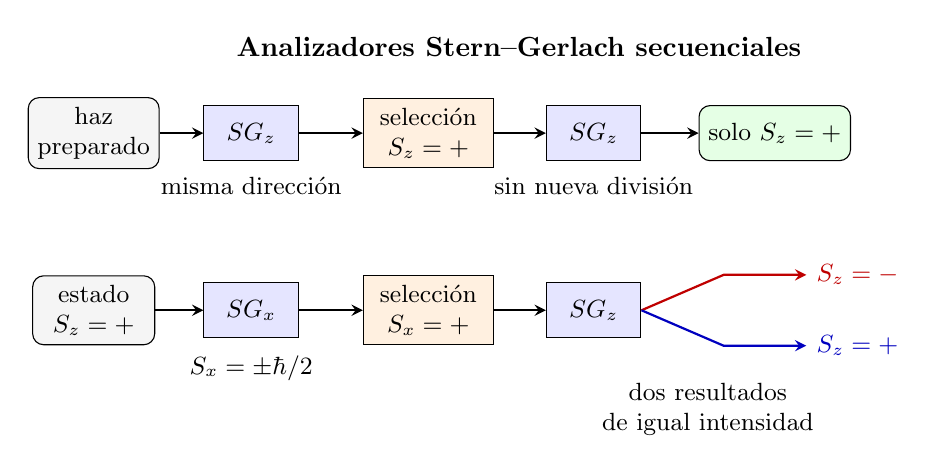
\begin{tikzpicture}[>=stealth, every node/.style={font=\small}]
        \node[font=\bfseries] at (5.4,2.15) {Analizadores Stern--Gerlach secuenciales};

        \node[draw,rounded corners,fill=gray!8,align=center,minimum width=1.55cm,minimum height=0.7cm] (source) at (0,1.05) {haz\\preparado};
        \node[draw,fill=blue!10,align=center,minimum width=1.2cm,minimum height=0.7cm] (sgz1) at (2.0,1.05) {$SG_z$};
        \node[draw,fill=orange!12,align=center,minimum width=1.65cm,minimum height=0.7cm] (selectz) at (4.25,1.05) {selección\\$S_z=+$};
        \node[draw,fill=blue!10,align=center,minimum width=1.2cm,minimum height=0.7cm] (sgz2) at (6.35,1.05) {$SG_z$};
        \node[draw,rounded corners,fill=green!10,align=center,minimum width=1.65cm,minimum height=0.7cm] (one) at (8.65,1.05) {solo $S_z=+$};
        \draw[->,thick] (source) -- (sgz1);
        \draw[->,thick] (sgz1) -- (selectz);
        \draw[->,thick] (selectz) -- (sgz2);
        \draw[->,thick] (sgz2) -- (one);
        \node[below] at (2.0,0.62) {misma dirección};
        \node[below] at (6.35,0.62) {sin nueva división};

        \node[draw,rounded corners,fill=gray!8,align=center,minimum width=1.55cm,minimum height=0.7cm] (prepared) at (0,-1.2) {estado\\$S_z=+$};
        \node[draw,fill=blue!10,align=center,minimum width=1.2cm,minimum height=0.7cm] (sgx) at (2.0,-1.2) {$SG_x$};
        \node[draw,fill=orange!12,align=center,minimum width=1.65cm,minimum height=0.7cm] (selectx) at (4.25,-1.2) {selección\\$S_x=+$};
        \node[draw,fill=blue!10,align=center,minimum width=1.2cm,minimum height=0.7cm] (sgz3) at (6.35,-1.2) {$SG_z$};
        \draw[->,thick] (prepared) -- (sgx);
        \draw[->,thick] (sgx) -- (selectx);
        \draw[->,thick] (selectx) -- (sgz3);
        \draw[->,thick,red!75!black] (sgz3.east) -- (8.0,-0.75) -- (9.05,-0.75) node[right] {$S_z=-$};
        \draw[->,thick,blue!75!black] (sgz3.east) -- (8.0,-1.65) -- (9.05,-1.65) node[right] {$S_z=+$};
        \node[below] at (2.0,-1.65) {$S_x=\pm\hbar/2$};
        \node[below,align=center] at (7.8,-2.0) {dos resultados\\de igual intensidad};
    \end{tikzpicture}
    \caption{Dos secuencias de analizadores: repetir una medición de $S_z$ conserva el resultado seleccionado; intercalar una medición de $S_x$ permite luego obtener ambos valores de $S_z$.}
    \label{fig:secuencia-sg}
\end{figure}